% !TEX root = ../thesis-example.tex
%
\chapter{fMRI and functional connectivity }
\label{sec:fmri}

\section{Structural and functional magnetic resonance imaging}
\label{sec:fmri:fmri}

\subsection{Magnetic resonance imaging (MRI)}
\label{sec:fmri:fmri:mri}

Magnetic resonance imaging (MRI) is probably the \q{most important imaging advance since the introduction of X-rays by Conrad Röntgen in 1895} \citep{logothetis_what_2008}. Indeed, the emergence of MRI has indeed marked the beginning of a new era in diagnostic medicine and basic research. MRI is based upon nuclear magnetic resonance, the physical phenomenon by which nuclei placed in an external magnetic field absorb and re-emit radio-frequency energy. MRI is the technique of choice for imaging brain structure. Indeed, magnetic properties of hydrogen nuclei vary with the biological tissue in which they are. For example, the rate of spin relaxation (i.e. how quickly spins "forget" the direction in which they are oriented) is not the same between gray and white matter, which thus makes it possible to construct detailed images of the brain at any location and orientation with sub-millimeter resolution.

\subsection{Functional MRI (fMRI)}
\label{sec:fmri:fmri:fmri}

Functional MRI (fMRI), built on the earlier concept of MRI, is a technique for measuring hemodynamic changes (i.e. blood flow dynamic) in the brain due to changing neural activity. Compared to structural MRI, the brain is scanned at lower spatial resolution (2-3 mm) but at a higher temporal resolution (typically a few seconds). Specifically, fMRI relies on the fact that hemoglobin in blood slightly distorts the magnetic resonance properties of hydrogen nuclei in its vicinity, and the amount of magnetic distortion changes depending on whether the hemoglobin has oxygen bound to it. For example, when neurons of a specific brain area become active, local blood flow to this region increase, and oxygen-rich (oxygenated) blood displaces oxygen-depleted (deoxygenated) blood around 2 seconds later (a phenomenon known as the hemodynamic response). These changes in the concentration of oxygen and blood flow lead to localized blood oxygenation level-dependent (BOLD) changes in the magnetic resonance signal. It is generally accepted that, in most brain regions, the fMRI signal is coupled to the level of excitatory and inhibitory synaptic transmission and therefore reflect the level of information processing \citep{logothetis_what_2008}.

\subsection{Task-based and resting-state paradigms}
\label{sec:fmri:fmri:paradigm}

Traditionally, fMRI has been used to produce maps of task-dependent brain function using block or event-related designs, which are based on the subtraction paradigm. In such designs, one infers the level of activation of certain brain areas by looking at the relative changes from baseline (resting or control condition) in the BOLD signal during the performance of a task or in response to a stimulus. During these designs, participants are instructed to perform specific tasks, which are generally designed to target a single brain function such as vision, attention, memory, emotion recognition and so on. These paradigms have allowed brain science to take giant strides, in particular on the issue of linking brain areas with specific functions (which was in the past only possible by studying cerebral lesions).
More recently, there has been a growing interest in the application of resting-state fMRI (RS-fMRI). Indeed, soon after the development of fMRI, Biswal and colleagues observed that the resting brain is not silent but contains information about its functional organization \citep{biswal_functional_1995}. Specifically, they reported that, during rest, time courses of low frequency fluctuations (<0.1 Hz) in somatomotor brain areas, showed a high degree of temporal correlation. They argued that this correlation, which may arise from fluctuations in blood oxygenation or flow, is a manifestation of functional connectivity of the brain. Although at the time Biswal’s seminal observation was mostly disregarded, it laid the basis for the now widely-used resting-state fMRI paradigm, which measures how different regions of the brain communicate while participants are not performing any active task. Although both resting-state and task-related designs measures BOLD signal, there are several major differences between the two, which are reported in Table \ref{tab:method:fMRI-paradigm}.

\begin{table}[]
\centering
\caption[Key differences between task-based fMRI and resting-state fMRI]{Key differences between task-based fMRI and resting-state fMRI. Modified from \citet{smitha_resting_2017}}
\label{tab:method:fMRI-paradigm}
\resizebox{\textwidth}{!}{%
\begin{tabularx}{\textwidth}{XXX}
\toprule
                      & Task-based fMRI                                                                                                                                          & Resting-state fMRI                                                                                                               \\ \midrule
Design                & Analyses of the relative changes from baseline in the BOLD signal during a task or in response to a stimulus & Analyses of the spontaneous BOLD signal in the absence of any explicit task or input \\
Energy consumption    & Task-specific increase in neuronal metabolism are less than 5\%                                             & 60–80\% of brain’s energy is consumed during resting state                                                                       \\
Brain areas           & The focus is only on a very small fraction of the brain’s overall activity                                   & The focus is on large-scale brain networks                                                                                       \\
Signal-to-noise ratio & Low since 80\% of the BOLD modulation is discarded as noise                                            & Good since it takes the overall spontaneous low frequency fluctuations               \\
Patient cooperation   & Patient cooperation is essential                                                                                                                         & Pediatric, psychiatric and even comatose patients can do\\   RS-fMRI                     \\
Duration              & Requires a large number of repetitions                                                                                                                   & Usually 6 to 10 minutes                                                                                                          \\ \bottomrule
\end{tabularx}%
}
\end{table}

\section{Functional connectivity}
\label{sec:fmri:fc}

\subsection{Overview}
\label{sec:fmri:fc:overview}

Functional connectivity can be defined as \q{the temporal dependence of neuronal activity patterns of anatomically separated brain regions} \citep{van_den_heuvel_exploring_2010}. It can be measured as long-range synchronization of the EEG, magneto-encephalography (MEG), or other dynamic brain signals. Applied to fMRI, functional connectivity reflects the temporal correlation of low frequency (<1 Hz) BOLD spontaneous fluctuations in spatially distinct brain regions (Figure \ref{fig:methods:fcmri}). Although the true neuronal basis of these slow BOLD fluctuations is not yet fully understood, there is converging evidence that they result from co-activation in the underlying spontaneous neuronal activation patterns. As a consequence, they are thought to reflect functional communication between brain areas. There are also several evidences that spontaneous BOLD fluctuations are partly constrained by anatomic connectivity \citep{van_dijk_intrinsic_2010}.
In more practical terms, these intrinsic BOLD fluctuations are nearly always measured at rest in order to minimize task-evoked effect. Resting-state fMRI has also the advantage of being quite simple to implement. For that reason, functional connectivity resting-state MRI has become the technique of choice to study the intrinsic functional organization of the brain in healthy individuals across a variety of vigilance states (such as sleep) but also in patients (e.g. comatose and psychiatric patients).

\begin{figure}[htb]
	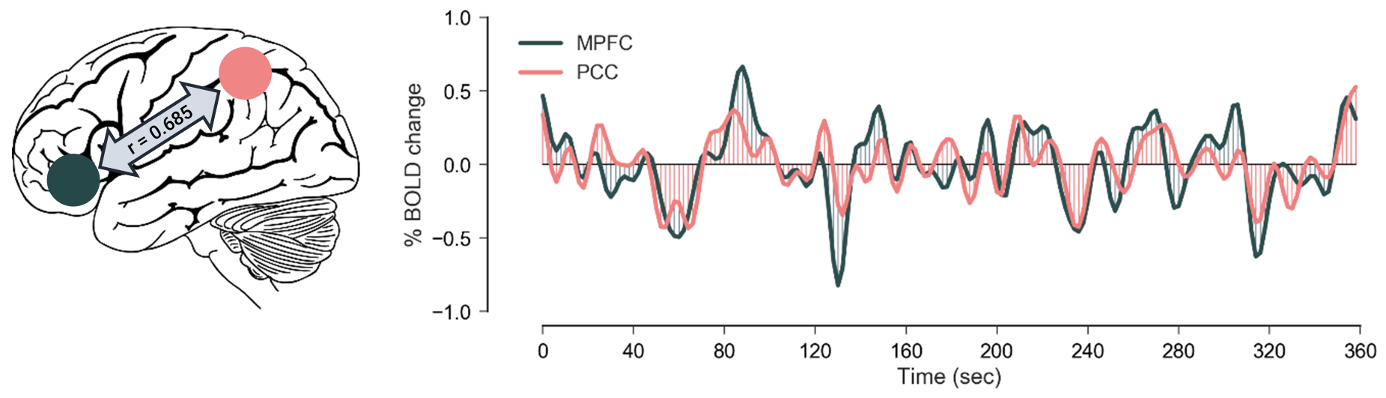
\includegraphics[width=\textwidth]{Fig/Methods/fMRI_temporal_correlation/fMRI_temporal_correlation.png}
	\caption[The basic strategy of functional connectivity MRI]{The basic strategy of functional connectivity MRI. The basis of functional connectivity is that spontaneous BOLD fluctuations measured at rest are correlated between spatially distinct brain regions. In this example, spontaneous BOLD fluctuations in the medial prefrontal cortex (MPFC) and posterior cingulate cortex (PCC) are correlated (Pearson r = 0.685). These data come from a 6-min resting state scan acquired in a single individual on a 3-tesla MRI scanner.}
	\label{fig:methods:fcmri}
\end{figure}

\subsection{Large-scale brain networks}
\label{sec:fmri:fc:network}

A decade of resting-state fMRI research has revealed that the human brain is organized into several large-scale functionally-correlated brain networks, which are consistently found in healthy subjects, different stages of consciousness and across species \citep{fox_spontaneous_2007, yeo_organization_2011}. Because they are preferentially identified during resting-state fMRI, these networks are often referred to as resting-state networks (RSNs). They are comprised of different brain regions that each have their own task and function, but which are continuously exchanging information with each other. Remarkably, they closely match the topographies of functional responses obtained by task-related fMRI using typical sensory, motor, and cognitive paradigms.
The main functional networks of the human brain are depicted in Figure \ref{fig:methods:networks}. The visual and somatomotor networks include regions of the primary and secondary visual and sensory-motor cortex respectively. These two sensory networks are characterized by a clear coupling between anatomic and functional connectivity \citep{van_dijk_intrinsic_2010}. Next, come the so-called task-positive networks, namely the frontoparietal (FP; sometimes referred to as executive, or control) network, the dorsal attention network (DAN), and the salience network. They are all involved in attentional processes. For instance, the DAN is thought to support selective attention to sensory features of the environment, while the salience network is involved in monitoring the salience of external inputs and internal brain events. There is emerging evidence that the FP network, originally thought to be involved in the selection of sensory contents by attention, may also orchestrate the interactions between other networks \citep{christoff_mind-wandering_2016}.

\begin{figure}[htb]
	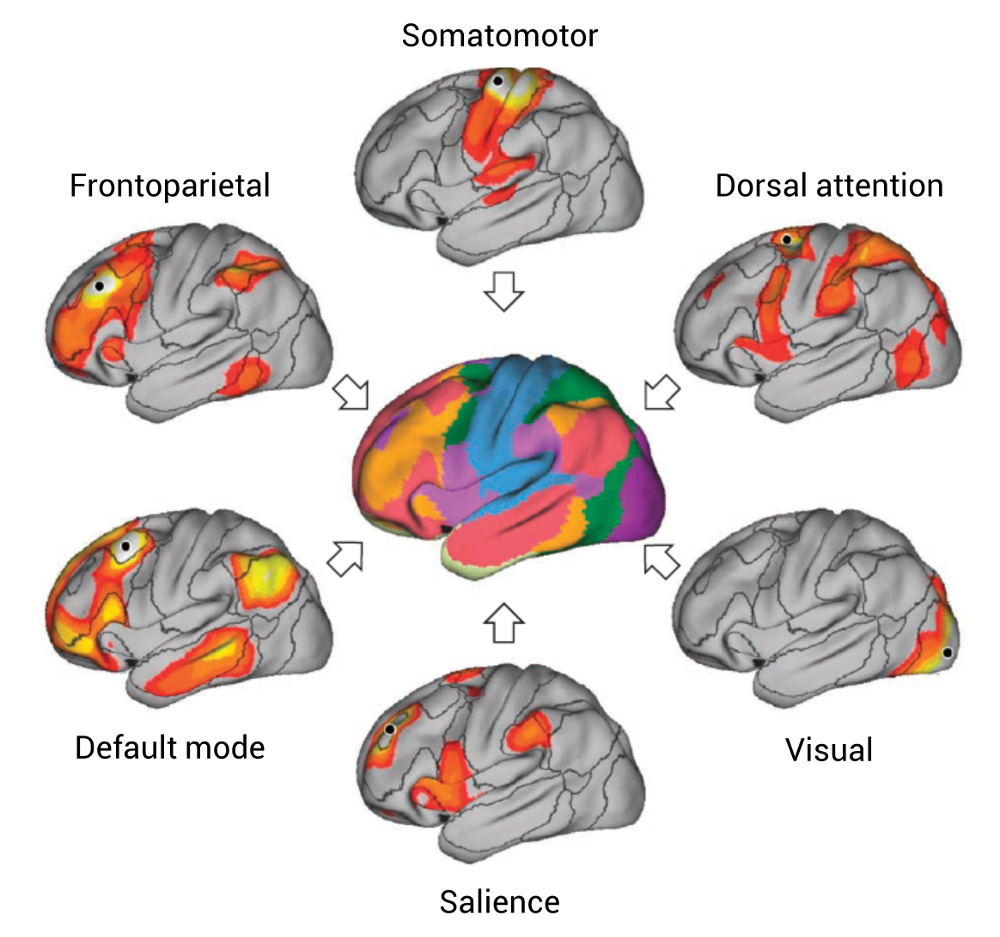
\includegraphics[width=\textwidth]{Fig/Methods/fMRI_Networks/fMRI_Networks.png}
	\caption[Large-scale brain networks]{Large-scale brain networks identified with resting-state functional connectivity fMRI. Outer maps show the functional connectivity maps for a single seed region (black circle) placed in a different cortical region, obtained using resting-state fMRI data in 1000 subjects. Center map show a composite estimate of the networks using an analytical approach to parcellate cortical regions into their most dominant network. Originally published in \citet{buckner_opportunities_2013}}
	\label{fig:methods:networks}
\end{figure}

Finally, the last and perhaps most investigated brain network is the default mode network (DMN, sometimes referred to as task-negative network), which was originally identified as a set of brain areas consistently deactivated across a range of externally oriented tasks \citep{raichle_default_2001}. It has been linked to internal mental processes, such as introspection, mind-wandering but also episodic memory retrieval and autobiographical future thinking. The DMN includes several subsystems which are supposedly involved in different functional roles  (Figure \ref{fig:methods:dmn}; \citealp{andrews-hanna_functional-anatomic_2010}). The DMN is probably one of the more robust RSN and has been identified across several brain states, including NREM and REM sleep \citep{horovitz_decoupling_2009, larson-prior_cortical_2009, larson-prior_modulation_2011, wu_variations_2012}. Recently, some authors have postulated that the DMN might be involved in the production and/or encoding of dreams (see section \ref{sec:dream-research:attempts:dmn}).

\begin{figure}[htb]
	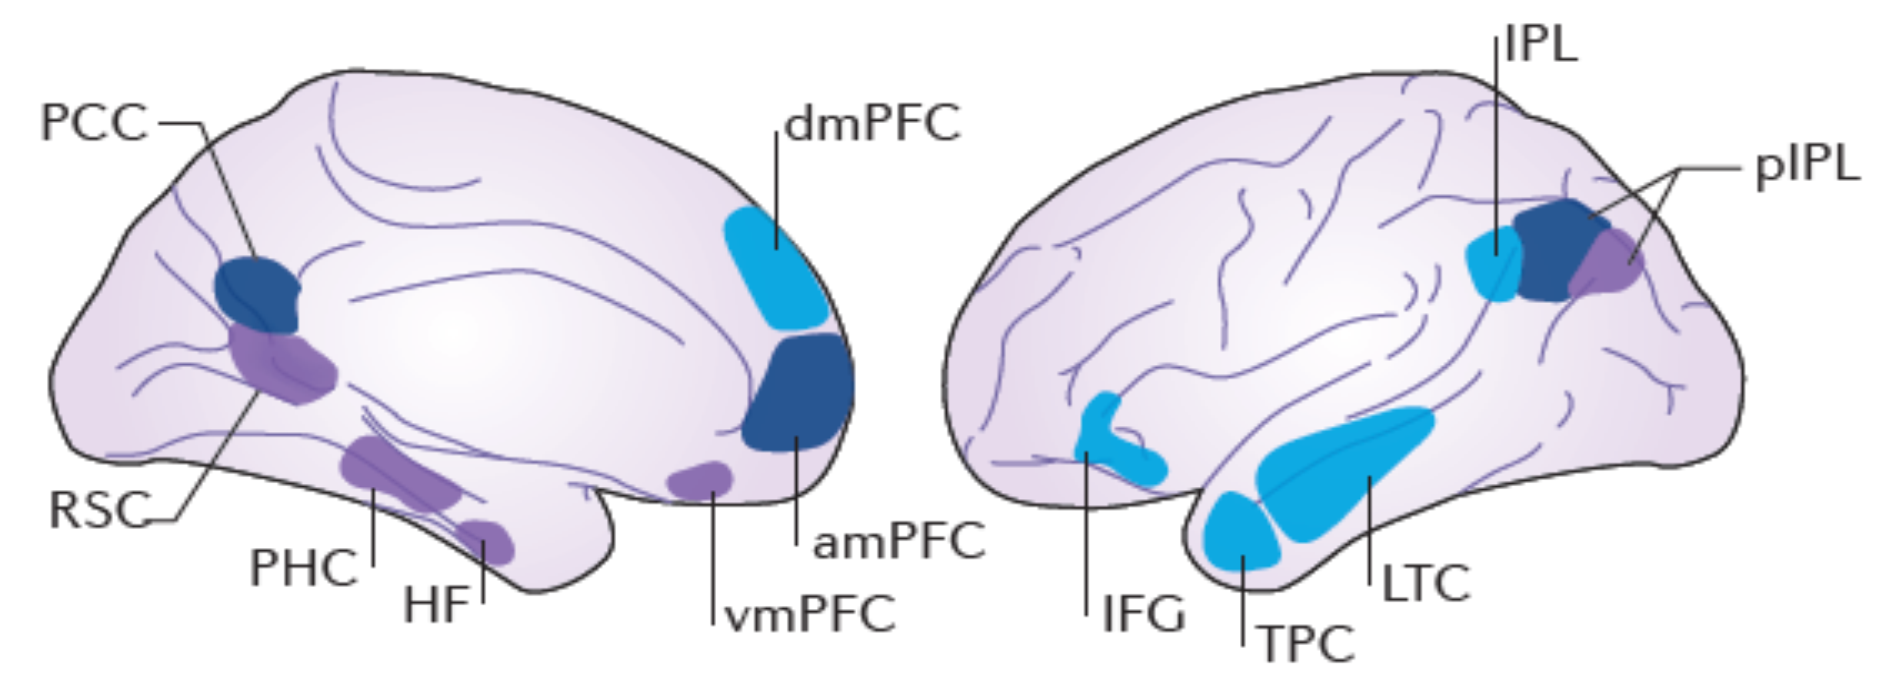
\includegraphics[width=\textwidth]{Fig/Methods/fMRI_DMN/Intro_DMN.png}
	\caption[The default mode network and its subcomponents]{The default mode network and its subcomponents. The DMN is centered on the medial prefrontal cortex (MPFC), the medial parietal cortex and the lateral parietal cortex, and extends into the temporal lobe and lateral prefrontal cortex. Three subcomponents within the DMN have been identified. The first, the core DMN subsystem (deep blue) includes the MPFC, posterior cingulate cortex (PCC) and posterior inferior parietal lobule (pIPL). It is characterized by its hub-like properties and its contributions to internally oriented cognition. The second subcomponent (purple), which is known for its roles in memory and mental simulation, is centered on the medial temporal lobe (MTL), and includes as well the hippocampal formation (HF) and parahippocampal cortex (PHC). The third subcomponent (cyan) extends more dorsally and includes the dorsomedial prefrontal cortex (dmPFC), the lateral temporal cortex (LTC), the temporopolar cortex (TPC) and parts of the inferior frontal gyrus (IFG). It seems to be linked to a wide range of functions, including mentalizing, conceptual processing and emotional processing. Originally published in \citet{christoff_mind-wandering_2016}.}
	\label{fig:methods:dmn}
\end{figure}

\subsection{Anti-correlations between networks}
\label{sec:fmri:fc:anti-correl}

\citet{fox_human_2005} reported that the DMN is negatively coupled (anti-correlated) to brain networks involved in focused external visual attention (i.e. mainly the DAN). In other words, when the spontaneous BOLD fluctuations increase in the DMN, they decrease in the DAN. This dynamic interplay between two large, spatially distributed networks representing a priori opposing components of our mental lives (the DMN is involved in internal mental processes, while the DAN is involved in external attention) may \q{mark a fundamental feature of brain organization that had not been appreciated by earlier techniques} \citep{buckner_opportunities_2013}. Remarkably, a decrease anti-correlation between the DMN and the DAN has been consistently reported in a variety of altered vigilance states such as during NREM sleep (review in \citealp{picchioni_sleep_2013}) and after total sleep deprivation \citep{de_havas_sleep_2012}. This suggests that anti-correlation between these networks is an essential part of the brain normal functional organization.

\section{Resting-state fMRI data analysis}
\label{sec:fmri:rs}

The aim of this section is to provide a brief overview of the numerous processing steps that must be performed to go from the raw structural and functional MRI images to the group-level statistical analysis. These steps are summarized in Figure \ref{fig:methods:fmri-pipeline}.

\subsection{Preprocessing}
\label{sec:fmri:rs:preproc}

Steps in the spatial preprocessing of task-related and resting state fMRI data are similar. The first step is usually slice-timing correction, which aims at correcting temporal offset between slices within a repetition time by applying a temporal data interpolation to each voxel of the brain. Indeed, an fMRI scanner typically requires 2 seconds (i.e. repetition time or TR) to construct a full 3D brain volume by slicing the brain into multiple 2D layers (acquired either in ascending or interleaved order). Consequently, the BOLD signal (hemodynamic response) acquired in the last slice (late in the TR) peaks earlier than those in the slices acquired early in TR, even though the underlying activity is identical. Slice-timing correction applies a temporal data interpolation to each voxel of the brain in order to reconstruct a signal as if all the slices within a TR were acquired at the same exact time point.
The second main step is the coregistration which refers to the alignment of functional and structural images from the same subject to map functional information into anatomical space. In layman’s term, this step ensures that the brain images acquired from a single individual are always in the same position and space. This step is particularly important in resting-state fMRI due to the global effect of head movements on spontaneous BOLD fluctuations.
Next comes normalization, which refers to the spatial transformation of individual brains into a common space (typically Montreal Neurological Institute (MNI) space), a step crucial in order to make brain volumes acquired in different subject with different brain morphologies comparable to each other. A temporal filtering is sometimes applied to remove or attenuate frequencies within the raw signal that are not of interest. For instance, as functional connectivity fMRI studies the spontaneous low-frequency BOLD fluctuations, a bandpass filter on frequencies between 0.01 Hz - 0.1 Hz is usually applied. Finally, the last preprocessing step is generally the spatial smoothing, which aims at further increasing the signal-to-noise ratio by filtering out high frequency regions. Smoothing is a prerequisite to parametric statistical analysis (such as the Gaussian random fields) which assume that data are well-modeled by a normal distribution, however, there is a controversy as to the role of smoothing in resting-state fMRI (and notably graph analysis) in which increased spatial dependency introduced by smoothing might confound local connectivity strength \citep{hayasaka_comparison_2010}.

\begin{figure}[htb]
	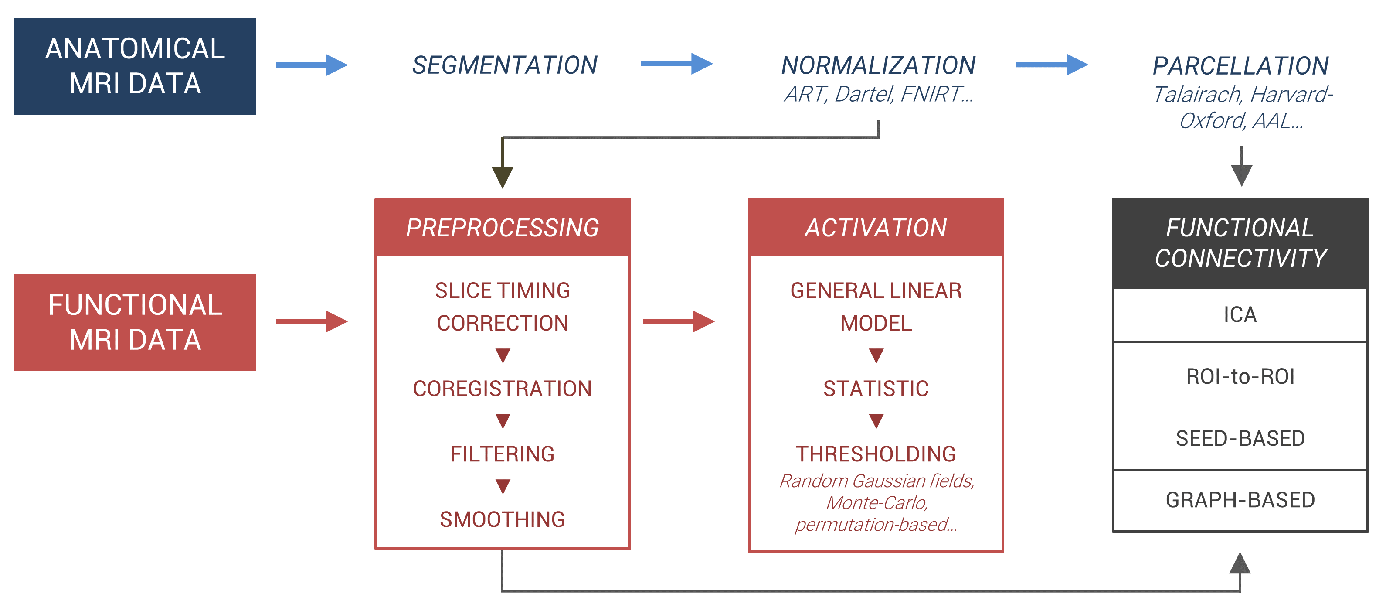
\includegraphics[width=\textwidth]{Fig/Methods/fMRI_pipeline/fMRI_pipeline_perso.png}
	\caption[Overview of the fMRI processing pipeline]{Overview of the fMRI processing pipeline. ICA = independent component analysis, a computational method for separating a multivariate signal into additive subcomponents (typically distinct brain networks). ROI = regions of interests. Adapted from an original idea of Oussama Abdoun.}
	\label{fig:methods:fmri-pipeline}
\end{figure}

\subsection{Functional connectivity analysis}
\label{sec:fmri:rs:analysis}

There are three prominent methods to analyze preprocessed resting-state fMRI data (Figure \ref{fig:methods:ana-methods}). The first one is independent component analysis (ICA), which is a statistical method for separating a multivariate signal into additive subcomponents. Applied to brain functional connectivity data, it allows for example to separate distinct brain networks, without making any kind of initial assumptions \citep{beckmann_investigations_2005}. Because it requires no a priori defined regions of interests (ROIs), it can be quite easily implemented to identify brain networks or to remove noisy components of the signal (e.g. physiological noise, scanner drift). The second approach is based on a priori defined cluster of voxels (referred to as seeds, or ROIs). In this case, the signal from a specific seed is correlated either with all the other voxels of the brain (voxel-to-voxel approach) or others ROI (ROI-to-ROI approach). The ROI-to-ROI method is particularly well-suited to analyze within and between networks interactions, provided that the ROIs are defined a priori (for example using an ICA or a brain atlas). Finally, an emerging method in resting-state fMRI analysis is graph theory, which studies the spatio-temporal properties of brain networks using mathematical tools \citep{bullmore_complex_2009}.

\begin{figure}[htb]
	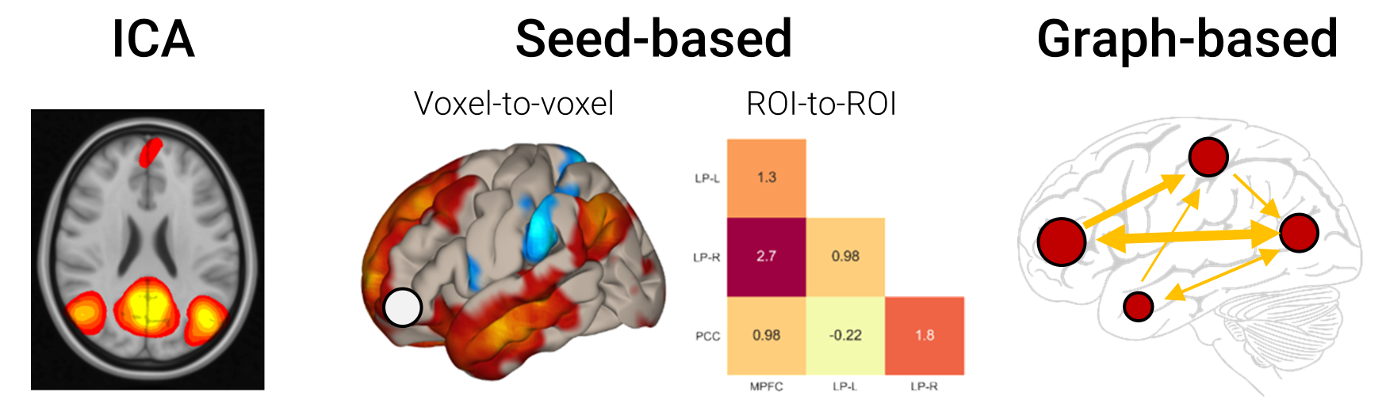
\includegraphics[width=\textwidth]{Fig/Methods/fMRI_seed_graph_ica/fMRI_seed_graph_ica.png}
	\caption[The three main methods of resting-state fMRI data analysis]{The three main methods of resting-state fMRI data analysis. 1) ICA is a highly data-driven method which is typically used to identify brain networks (in this example, the core regions of the DMN) or remove noisy components. 2) Seed-based connectivity requires one or several regions of interests (ROIs) to be a priori defined in order to compute the correlations between the seed regions and all the others voxels in the brain (voxel-to-voxel) or between specific ROIs (ROI-to-ROI). In this example, a symmetric correlation matrix was obtained by computing all the pairwise correlations within the DMN. 3) Graph-based connectivity studies the topological features of brain networks, which are defined in this context as a set of nodes (ROIs) linked by connections (edges). Using mathematical tools, several parameters can be computed such as the global efficiency and the level of modularity / clustering.}
	\label{fig:methods:ana-methods}
\end{figure}

\subsection{Combined EEG-fMRI recordings}
\label{sec:fmri:rs:eeg-fmri}

Simultaneous recording of EEG and MRI allow researchers to benefit from the excellent temporal resolution of EEG combined with the high spatial accuracy of fMRI. Applied to sleep, it allows for example to perform correlation between sleep features and stages (detected using classic EEG-based criteria), and BOLD-fMRI signal \citep{duyn_eeg-fmri_2012}. The EEG can also be used to detect online the different sleep stages, thus allowing the experimenter to decide when to launch an fMRI scan. Simultaneous EEG-fMRI is therefore a valuable tool for investigating brain function across the spectrum of vigilance states.
However, there are a number of technical challenges that need to be overcome in order to improve EEG-fMRI data acquisition. Most importantly, EEG signals acquired during simultaneous fMRI are affected by several artefacts, namely the gradient artefact (caused by the changing magnetic fields gradients required for fMRI) and the cardio-ballistic artefact (linked to cardiac pulsations). Fortunately, these artefacts can be almost entirely removed, a posteriori but also in real-time, using dedicated softwares or algorithms.
